\documentclass[tikz,border=2pt]{standalone}
\usepackage{amsmath,amssymb}
\usepackage{tikz}
\usetikzlibrary{arrows.meta}

\begin{document}
% A basis (b1, b2) of R^2 lays its own grid over the plane; every vector has exactly one
% address in that grid: w = 2 b1 + 1 b2.
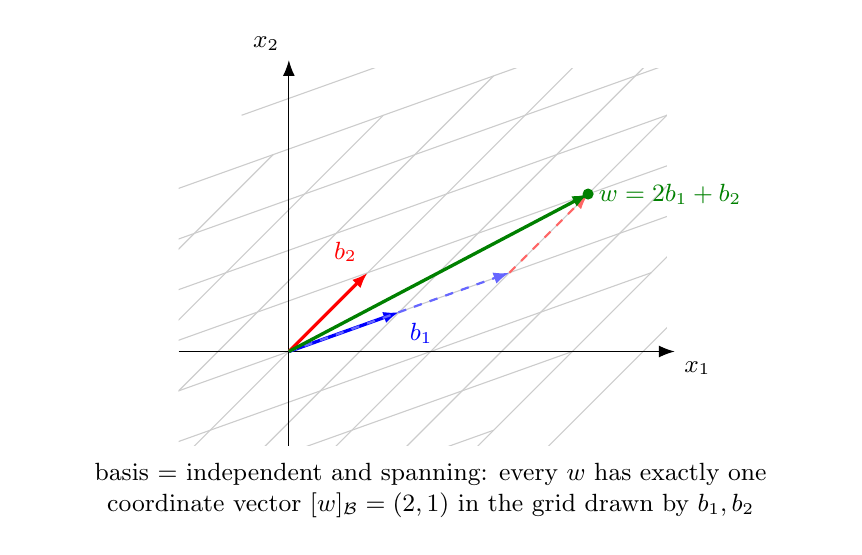
\begin{tikzpicture}[every node/.style={font=\small}, >={Latex[length=2mm]}]
	\begin{scope}
		\clip (-1.4,-1.2) rectangle (4.8,3.6);
		\foreach \i in {-3,...,5} {
			\draw[gray!40] ({\i*1.4-4},{\i*0.5-4}) -- ({\i*1.4+4},{\i*0.5+4});
			\draw[gray!40] ({\i-5.6},{\i-2}) -- ({\i+5.6},{\i+2});
		}
	\end{scope}
	\draw[->] (-1.4,0) -- (4.9,0) node[below right] {$x_1$};
	\draw[->] (0,-1.2) -- (0,3.7) node[above left] {$x_2$};
	\draw[->, blue, very thick] (0,0) -- (1.4,0.5) node[below right] {$b_1$};
	\draw[->, red, very thick] (0,0) -- (1,1) node[above left] {$b_2$};
	\draw[->, blue!60, thick, dashed] (0,0) -- (2.8,1.0);
	\draw[->, red!60, thick, dashed] (2.8,1.0) -- (3.8,2.0);
	\draw[->, green!50!black, very thick] (0,0) -- (3.8,2.0) node[right] {$w=2b_1+b_2$};
	\fill[green!50!black] (3.8,2.0) circle (2pt);
	\node[anchor=north, align=flush center, text width=10cm] at (1.8,-1.3) {basis = independent and spanning: every $w$ has exactly one coordinate vector $[w]_{\mathcal{B}}=(2,1)$ in the grid drawn by $b_1,b_2$};
\end{tikzpicture}
\end{document}
